\ifdefined\beamerclass
\else
    \def\beamerclass{beamer}
\fi
\documentclass[\beamerclass]{beamer}

\usepackage{pgfpages}
\mode<handout>{
  % \setbeamercolor{background canvas}{bg=black!20}
  \pgfpagesuselayout{2 on 1}[a4paper,border shrink=5mm]
}

\usepackage{lmodern}
\usepackage{listings}
\usepackage{amsmath}
\usepackage{bm}
\usepackage{textpos} % package for the positioning

\usepackage{pgf, tikz}
\usetikzlibrary{arrows, automata}

\usetheme{Copenhagen}
\hypersetup{pdfstartview={Fit}}
\lstset{basicstyle=\small\ttfamily,breaklines=true}

\usepackage[english]{babel}
\usepackage{algorithm}
\usepackage[noend]{algpseudocode}
\usepackage[utf8x]{inputenc}
\usepackage{graphicx}
\usepackage{hyperref}
%\graphicspath{{./images/}}
\usepackage{tikz}
\usetikzlibrary{shapes.geometric, arrows,chains}
\usepackage{booktabs,makecell,multirow,tabularx}
\usepackage{verbatim}
\renewcommand{\arraystretch}{1.2}
\renewcommand\theadfont{\normalfont\bfseries}
\usepackage{array}
\usepackage{listings}
\lstset{language=Java, showstringspaces=false}
\usepackage[normalem]{ulem}
\usepackage{bm}
\def\layersep{2.5cm}

\usepackage{xcolor}
%\usepackage{subfig}
\setbeamertemplate{caption}{\insertcaption}
\usepackage[caption=false]{subfig}
\usepackage{hyperref}
\usepackage{verbatim}
%\setbeamertemplate{caption}[numbered]%\numberwithin{figure}{section}
% Define block styles
\tikzstyle{decision} = [diamond, draw, fill=blue!20, 
    text width=4.5em, text badly centered, node distance=3cm, inner sep=0pt]
\tikzstyle{block} = [rectangle, draw, fill=blue!20, 
    text width=3em, text centered, rounded corners, minimum height=3em]
\tikzstyle{line} = [draw, -latex']
\tikzstyle{cloud} = [draw, ellipse, fill=red!20, node distance=3cm,
    minimum height=2em]
\tikzset{
  startstop/.style={
    rectangle, 
    rounded corners,
    minimum width=3cm, 
    minimum height=1cm,
    align=center, 
    draw=black, 
    fill=red!30
    },
  process/.style={
    rectangle, 
    minimum width=3cm, 
    minimum height=1cm, 
    align=center, 
    draw=black, 
    fill=blue!30
    },
  decision/.style={
    rectangle, 
    minimum width=3cm, 
    minimum height=1cm, align=center, 
    draw=black, 
    fill=green!30
    },
  arrow/.style={thick,->,>=stealth},
  dec/.style={
    ellipse, 
    align=center, 
    draw=black, 
    fill=green!30
    },
}
\tikzstyle{arrow} = [thick,->,>=stealth]

\tikzset{onslide/.code args={<#1>#2}{%
  \only<#1>{\pgfkeysalso{#2}} % \pgfkeysalso doesn't change the path
}}

\makeatletter
\newenvironment<>{btHighlight}[1][]
{\begin{onlyenv}#2\begingroup\tikzset{bt@Highlight@par/.style={#1}}\begin{lrbox}{\@tempboxa}}
{\end{lrbox}\bt@HL@box[bt@Highlight@par]{\@tempboxa}\endgroup\end{onlyenv}}

\newcommand<>\btHL[1][]{%
  \only#2{\begin{btHighlight}[#1]\bgroup\aftergroup\bt@HL@endenv}%
}
\def\bt@HL@endenv{%
  \end{btHighlight}%   
  \egroup
}
\newcommand{\bt@HL@box}[2][]{%
  \tikz[#1]{%
    \pgfpathrectangle{\pgfpoint{1pt}{0pt}}{\pgfpoint{\wd #2}{\ht #2}}%
    \pgfusepath{use as bounding box}%
    \node[anchor=base west, fill=orange!30,outer sep=0pt,inner xsep=1pt, inner ysep=0pt, rounded corners=3pt, minimum height=\ht\strutbox+1pt,#1]{\raisebox{1pt}{\strut}\strut\usebox{#2}};
  }%
}
\makeatother

\definecolor{darkblue}{RGB}{37,55,97}
\definecolor{mellowyellow}{RGB}{247,206,70}
\definecolor{almostwhite}{RGB}{254,255,255}
\definecolor{merrygreen}{RGB}{79,173,91}
\definecolor{funkyorange}{RGB}{240,154,56}

\addtobeamertemplate{footnote}{\hskip -2em}{}
\newcommand\blfootnote[1]{%
  \begingroup
  \renewcommand\thefootnote{}\footnote{#1}%
  \addtocounter{footnote}{-1}%
  \endgroup
}

\DeclareMathOperator{\softmax}{softmax}
\DeclareMathOperator{\ReLU}{ReLU}


%%%%%%%%%%%%%%%%%%%%%%%%%%%%%%%%%%%%%%%%%%%%%%
% Formatting for title page
\title[Visualisation]{Visualisation}
\author{Ethan Harris}  
\institute[]
{
  Vision, Learning and Control\\
  University of Southampton 
}
\date{}
\subject{Computer Science}
\useoutertheme{infolines}
\setbeamertemplate{headline}{} %remove headline
\setbeamertemplate{navigation symbols}{} %remove navigation symbols

%%%%%%%%%%%%%%%%%%%%%%%%%%%%%%%%%%%%%%%%%%%%%%
\begin{document}

\begin{frame}[plain]
  \begin{tikzpicture}[overlay, remember picture, shift={(current page.south west)},font={\fontfamily{Montserrat-TOsF}\selectfont}]
  \fill [mellowyellow,text=darkblue] (0,0) rectangle (\paperwidth, \paperheight);
  \draw (4,7) node [align=left,text=darkblue] {\Huge \begin{tabular}{l} \textbf{Maximise} \\ \textbf{Activations} \end{tabular}};
  \draw (11,1) node [align=left,text=darkblue] {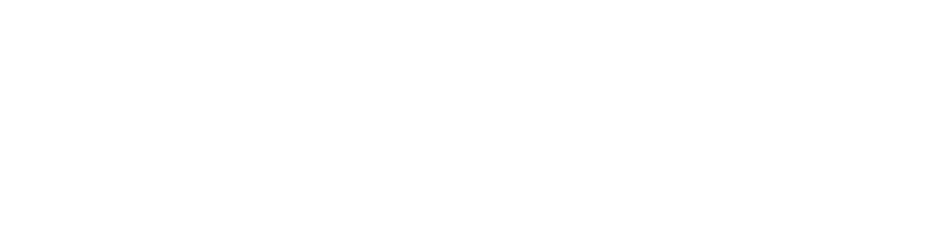
\includegraphics[scale=0.15]{vlc.png}};
  \end{tikzpicture}
\end{frame}


\begin{frame}
  \titlepage%\footnote{Some of the material in this lecture is based on Andrew Ng's lectures on Optimisation} %% \url{https://www.cs.toronto.edu/~tijmen/csc321/slides/lecture_slides_lec6.pdf }} 
\end{frame}

\begin{frame}\frametitle{Overview} 
\begin{itemize}
  \item The Electrophysical and Psychophysical Aspects of Vision
  \item Characterising Single Cells
  \item Feature Visualisation: Monkeys to Machines
  \begin{itemize}
      \item Decorrelation
      \item Reparameterisation
      \item Maximising: Cells, Layers, Predictions
  \end{itemize}
  \item Machines to Monkeys
\end{itemize}
\end{frame}

\begin{frame}\frametitle{Note} 
\begin{itemize}
  \item Feature visualisation article here: \url{https://distill.pub/2017/feature-visualization/}
  \item PyTorch implementations of key algorithms which generated the images can be found here: \url{https://github.com/pytorchbearer/visual}
\end{itemize}
\end{frame}

\begin{frame}\frametitle{The Electrophysical and Psychophysical Aspects of Vision} 
\begin{itemize}
  \item<+-> We want to know the function of the brains input that gives rise to some output
  \item<+-> Inputs - visual stimuli
  \begin{itemize}
      \item<+-> still images, moving stimuli, colour, greyscale, ...
  \end{itemize}
  \item<+-> Outputs - activations
  \begin{itemize}
      \item<+-> single cells, groups of cells, external actions, micro-electrode recordings, fMRI, ...
  \end{itemize}
\end{itemize}
\end{frame}

%%-------------------------------------------------------------%

\begin{frame}
  \frametitle{Characterising Single Cells}
  \begin{itemize}
      \item<+-> Using a micro-electrode recording from a cell, we can plot the \textbf{response curve} to a range of stimuli
      \item<+-> Need to restrict to some controlled stimuli space - colour? edge orientation?
  \end{itemize}
\end{frame}

\begin{frame}
  \frametitle{Case Study: Colour Opponency}
  \begin{itemize}
      \item<+-> Consider the baseline response (or spontaneous rate) of a cell to an empty visual field (i.e. constant grey-level across the retina)
      \item<+-> Now, we change the colour (wavelength) of the visual stimuli and measure the response
  \end{itemize}
\end{frame}

\begin{frame}
  \frametitle{De Valois: Analysis of Response Patterns of LGN Cells}
  \begin{itemize}
      \item<+-> Macaque Lateral Geniculate Nucleus (LGN) cells
  \end{itemize}
  \centering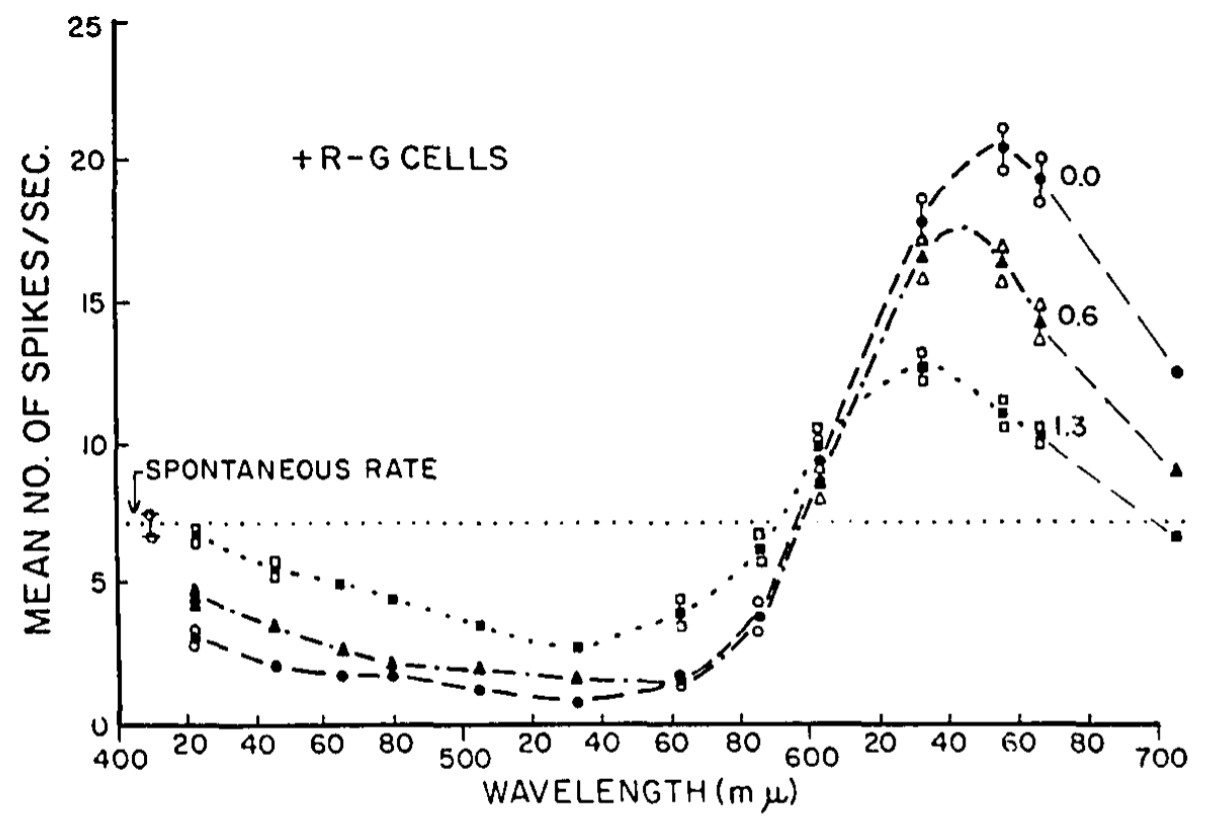
\includegraphics[width=7cm]{devalois.png}
  \begin{itemize}
      \item<+-> Opponent if the curve crosses the line - Non-opponent otherwise
      \item<+-> An analogous form of opponency can be defined - \textbf{spatial} opponency
      \item<+-> Cells which are both spatially opponent and colour opponent are called \textbf{double} opponent
  \end{itemize}
\end{frame}

\begin{frame}{Opponency in Deep Networks}
    \begin{itemize}
        \item<+-> Turns out both spatial and colour opponency happen in deep networks too!
        \item<+-> We measure in \textbf{exactly} the same way as we would in a Monkey - but on a much bigger scale
        \item<+-> More here: \url{https://github.com/ecs-vlc/opponency}
    \end{itemize}
    \centering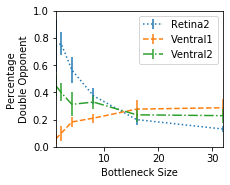
\includegraphics[width=5cm]{double_opponent.png}
\end{frame}

\begin{frame}{Feature Visualisation: Monkeys to Machines}
    \begin{itemize}
        \item<+-> We can also ask the question 'what most excites this cell?' in a deep network
        \item<+-> We've shown a range of stimuli and plotted a response curve as with the monkey
        \item<+-> Can we do something smarter?
        \item<+-> Gradient ascent - use the gradient information we have to `learn' the image which maximises the response of a particular cell or channel
    \end{itemize}
\end{frame}

\begin{frame}{Gradient Ascent}
    \centering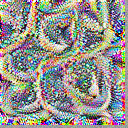
\includegraphics[width=5cm]{plain.png}
    \begin{itemize}
        \item<+-> Inception V3, Layer 6 - Noisy image - not very informative
        \item<+-> Gradient ascent makes an \textbf{uncorrelated} update in a \textbf{correlated} space - hence the crazy colours
    \end{itemize}
\end{frame}

\begin{frame}{Colour Correlation}
    \begin{itemize}
        \item<+-> Compute the RGB correlation statistics from ImageNet
        \item<+-> Correlate the colour channels of the input according to these statistics at each step - now the gradient update is over the \textbf{uncorrelated} parameters
        \item<+-> This type of trick is referred to as \textbf{re-paramterisation} or \textbf{preconditioning}
        \item<+-> The maxima don't change - but the loss surface does - some optima become more likely to be found
    \end{itemize}
\end{frame}

\begin{frame}{Colour Correlation}
    \centering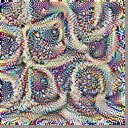
\includegraphics[width=5cm]{correlated.png}
    \begin{itemize}
        \item What can we do about the noise?
    \end{itemize}
\end{frame}

\begin{frame}{Frequency Penalisation}
    \begin{itemize}
        \item<+-> We can construct additional loss functions that penalise high frequencies
        \begin{itemize}
            \item Total variation, blur, L1 loss, ...
        \end{itemize}
        \item<+-> It's better - but we have other ways to improve optimisation procedures
    \end{itemize}
    \centering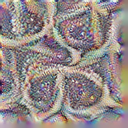
\includegraphics[width=5cm]{penalised.png}
\end{frame}

\begin{frame}{Augmentation}
    \begin{itemize}
        \item<+-> Randomly transform our image before each step
        \item parameters $\to$ correlation $\to$ frequency penalisation $\to$ augmentation $\to$ model
        \item<+-> We know the importance of correlation - what else is correlated in natural images?
    \end{itemize}
    \centering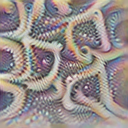
\includegraphics[width=5cm]{augmented.png}
\end{frame}

\begin{frame}{Fourier Space}
    \begin{itemize}
        \item<+-> Space! pixel values are correlated with their neighbours
        \item<+-> But how do we model spatial correlation?
        \item<+-> If a correlation is spatially consistent (i.e. it is constant over the extent of the image) then the Fourier coefficients are \textbf{independent}
        \item<+-> Think of a spatially consistent correlation as a convolution operation
        \item<+-> By the convolution theorem, this is a point-wise multiplication in Fourier space - it treats the coefficients independently
        \item<+-> The Fast Fourier Transform (FFT) is differentiable!
    \end{itemize}
\end{frame}

\begin{frame}{Fourier Space}
    \begin{itemize}
        \item Fourier coefficients $\to$ parameters $\to$ correlation $\to$ augmentation $\to$ model - frequency penalisation is turned off here
        \item That's better!
    \end{itemize}
    \centering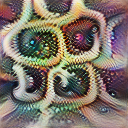
\includegraphics[width=5cm]{fourier.png}
\end{frame}

\begin{frame}{Maximising the Outputs}
    \begin{itemize}
        \item We could also maximise the outputs for a particular class
        \item Here's an Indian Elephant (class 385)
    \end{itemize}
    \centering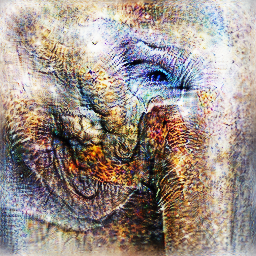
\includegraphics[width=5cm]{elephant.png}
\end{frame}

\begin{frame}{Maximising the Outputs}
    \begin{itemize}
        \item And a Grasshopper (class 311)
    \end{itemize}
    \centering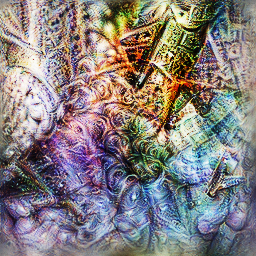
\includegraphics[width=5cm]{grasshopper.png}
\end{frame}

\begin{frame}{Maximising the Outputs}
    \begin{itemize}
        \item Or a Strawberry (class 949)
        \item You get the idea - deep neural networks don't learn about shape!
    \end{itemize}
    \centering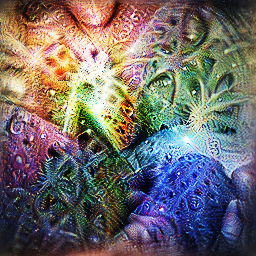
\includegraphics[width=5cm]{strawberry.png}
\end{frame}

\begin{frame}{Maximising the Interestingness}
    \begin{itemize}
        \item<+-> What if we maximise the sum of the squares of the outputs from a whole layer?
        \item<+-> DeepDream! - best results when we start with a real image and gradually increase the scale through training
    \end{itemize}
\end{frame}

\begin{frame}{Mona Lisa}
    \centering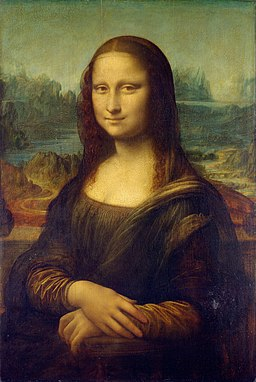
\includegraphics[width=5cm]{mona_lisa.jpg}
\end{frame}

\begin{frame}{Mona Lisa}
    \centering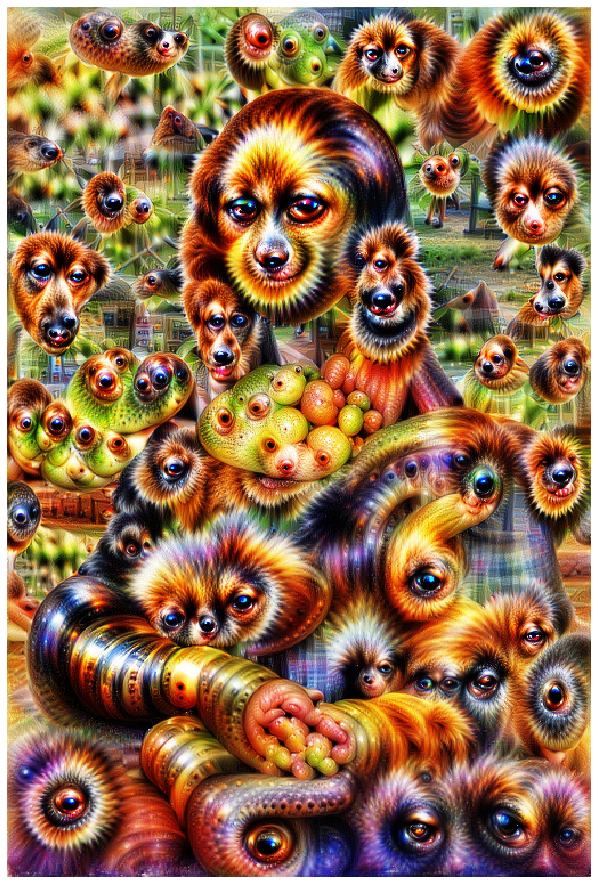
\includegraphics[width=5cm]{mona_lisa_dream.png}
\end{frame}

\begin{frame}{And Back to Monkeys}
    \begin{itemize}
        \item<+-> So we've seen how we can get great visualisations of deep networks
        \item<+-> Much more informative than just looking at single cells
        \item<+-> What's stopping us from doing this in a real brain?
        \item<+-> Nothing! - gradient free optimisers exist - we could use a genetic algorithm
    \end{itemize}
\end{frame}

\begin{frame}{XDREAM}
    \begin{itemize}
        \item Monkey + Genetic Algorithm + Deep Generative Network 
    \end{itemize}
    \centering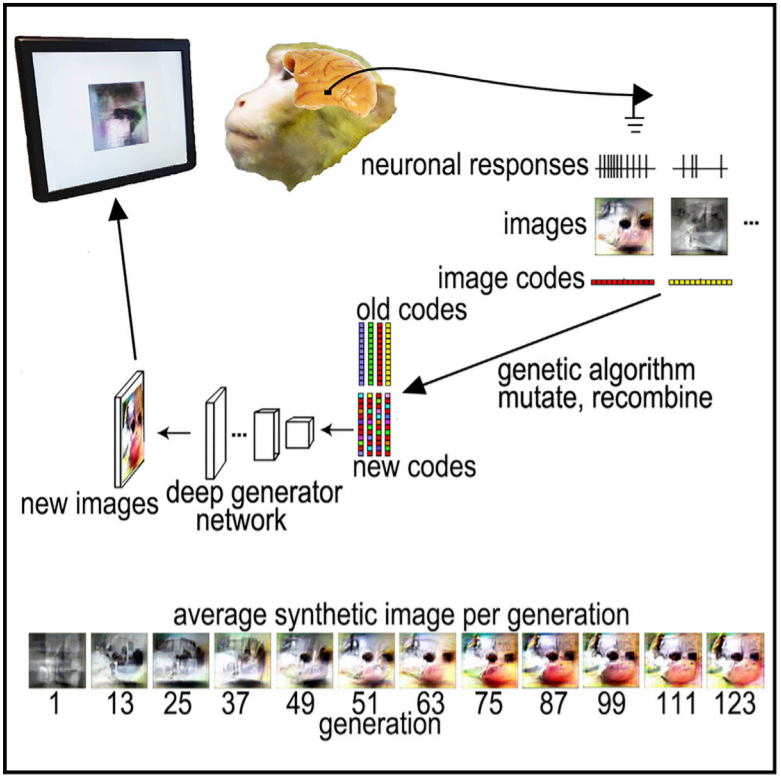
\includegraphics[width=5cm]{xdreamplot.png}
\end{frame}

\begin{frame}{XDREAM}
    \begin{itemize}
        \item Neurons in the Inferior Temporal cortex (AKA the `what' pathway)
    \end{itemize}
    \centering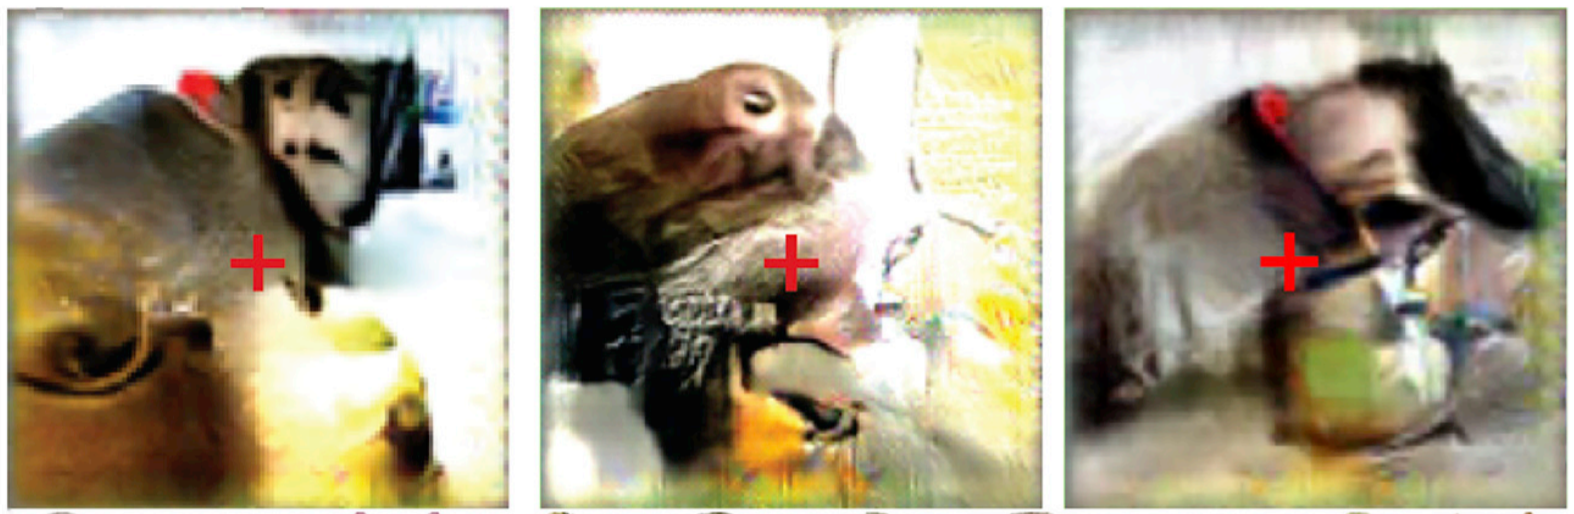
\includegraphics[width=10cm]{xdream.png}
\end{frame}

\begin{frame}{Closing Remarks}
    \begin{itemize}
        \item<+-> Finding the stimuli which maximise the response of single cells has a long history in Neuroscience
        \item<+-> Applying that idea to deep learning we get a way to understand what each `cell' has learned
        \item<+-> But be careful - feature visualisation is more of an art than a science - it isn't a completely solved problem
        \item<+-> Lessons and tools from deep learning can feed back in to Neuroscience, helping us to understand \textbf{much} more complex parts of the brain
        \item<+-> Maybe deep models and brains aren't so different after all!
    \end{itemize}
\end{frame}


\end{document}
